\documentclass[border=4pt]{standalone}
\usepackage{tikz}
\usetikzlibrary{arrows,arrows.spaced,positioning}
\begin{document}
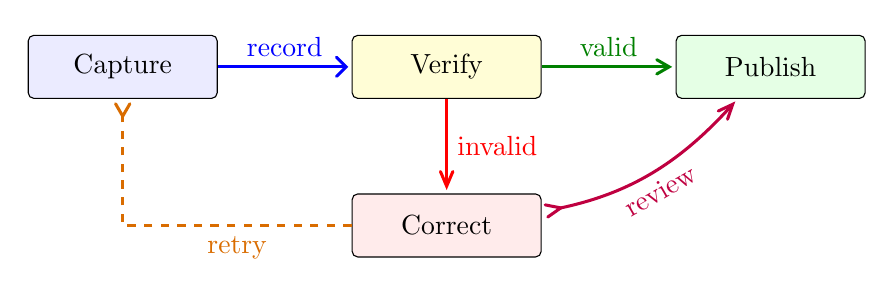
\begin{tikzpicture}[
  node distance=12mm and 17mm,
  stage/.style={draw,rounded corners=2pt,minimum width=24mm,minimum height=8mm,align=center},
  route/.style={line width=1.1pt}
]
  \node[stage,fill=blue!8] (capture) {Capture};
  \node[stage,fill=yellow!16,right=of capture] (verify) {Verify};
  \node[stage,fill=green!10,right=of verify] (publish) {Publish};
  \node[stage,fill=red!8,below=of verify] (correct) {Correct};

  \draw[route,blue,-{spaced angle 90}]
    (capture) -- node[above]{record} (verify);
  \draw[route,green!50!black,-{spaced angle 60}]
    (verify) -- node[above]{valid} (publish);
  \draw[route,red,-{spaced angle 45}]
    (verify) -- node[right]{invalid} (correct);
  \draw[route,dashed,orange!85!black,-{spaced angle 60 reversed}]
    (correct.west) -| node[pos=.25,below]{retry} (capture.south);
  \draw[route,purple,{spaced angle 45 reversed}-{spaced angle 45}]
    (correct) to[bend right=18] node[below,sloped]{review} (publish);
\end{tikzpicture}
\end{document}
